\documentclass[12pt,fleqn]{article}\usepackage{../../common}
\begin{document}
Materyel Mekaniği - 5

Bu derste kirişler ve makaskirişleri üstdüşüm ile birleştirip hem eksenel hem
eksene dik kuvvetler ile nasıl hesap yapabileceğimizi göreceğiz. Daha sonra bu
yeni parça türü bir şasi içinde biraraya koyulup daha çetrefil yapılar analiz
edilecek. Ama önce döndürme kavramını görelim.

Dönüş (Rotation)

Alttaki gibi bir kiriş düşünelim,

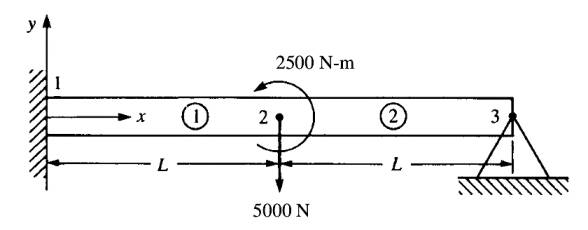
\includegraphics[width=20em]{phy_020_strs_06_01.jpg}

Daha önce bu tür bir kiriş üzerinde eksenel yöndeki kuvvetler ve yer
değişimlerinin ilişkisini

$$
\left[\begin{array}{c}
f'_{1x} \\ f'_{2x}
\end{array}\right] =
\frac{AE}{L}
\left[\begin{array}{cc}
1 & -1 \\ -1 & 1
\end{array}\right]
\left[\begin{array}{c}
u'_1 \\ u'_2
\end{array}\right]
\mlabel{1}
$$

olarak göstermiştik. Üstteki formül kirişin yerel, kendisine has kordinat
sistemini baz alıyor. Eğer üstteki değişkenleri global kordinat sistemine
eşlemek, yansıtmak istiyorsak o zaman sistemi resimdeki $\theta$ kadar döndürmemiz
gerekiyor. Döndürme işlemi genel olarak iki boyuttaki bir $[u, v]$ vektörü için
[1, sf. 85]

$$
\left[\begin{array}{c}
u' \\ v'
\end{array}\right] =
\left[\begin{array}{cc}
C & S \\ -S & C
\end{array}\right]
\left[\begin{array}{c}
u \\ v
\end{array}\right]
\mlabel{2}
$$

ile yapılır, ki $C = \cos\theta$, $S = \sin\theta$.

Fakat unutmayalım tek eksenlikten çıktığımız zaman kirişin her ucunda iki
serbestlik derecesi vardır, her uç $u,v$ yönünde yer değişim yaşayabilir,
bunları $u_1,v_1$ ve $u_2,v_2$ diye gösterebiliriz. O zaman dönüş hesabı

$$
\left[\begin{array}{c}
u'_1 \\ v'_1 \\ u'_2 \\ v'_2
\end{array}\right] =
\left[\begin{array}{cccc}
C & S & 0 & 0 \\
-S & C & 0 & 0 \\
0 & 0 & C & S \\
0 & 0 & -S & C 
\end{array}\right]
\left[\begin{array}{c}
u_1 \\ v_1 \\ u_2 \\ v_2
\end{array}\right]
$$

İlerlemeden önce iki üstteki dönüş matrisi, $T$ diyelim, hakkında ilginç bir
ispatı verelim, ileride lazım olacak. Acaba $T^T = T^{-1}$ ifadesi doğru mudur?
Bu aynı zamanda [1] kitabındaki 3.28 probleminin de cevabı. İspat için $T T^T$
çarpımını yapabiliriz, eğer birim (identity) matrisi elde edersek ispat tamam
demektir.

$$
T = 
\left[\begin{array}{cccc}
C & S & 0 & 0 \\
-S & C & 0 & 0 \\
0 & 0 & C & S \\
0 & 0 & -S & C 
\end{array}\right], \quad
T^T = 
\left[\begin{array}{cccc}
C & -S & 0 & 0 \\
S & C & 0 & 0 \\
0 & 0 & C & -S \\
0 & 0 & S & C 
\end{array}\right]
$$

Çarpımı \verb!sympy! ile yapalım,

\begin{minted}[fontsize=\footnotesize]{python}
from sympy import symbols, pprint, latex
from sympy.matrices import Matrix
C,S = symbols("C,S")
T = Matrix([[C,S,0,0],[-S,C,0,0],[0,0,C,S],[0,0,-S,C]])
Tprime = Matrix([[C,-S,0,0],[S,C,0,0],[0,0,C,-S],[0,0,S,C]])
print (latex(T * Tprime)[:60],'...')
\end{minted}

\begin{verbatim}
\left[\begin{matrix}C^{2} + S^{2} & 0 & 0 & 0\\0 & C^{2} + S ...
\end{verbatim}

Yani,
  
$$
\left[\begin{matrix}C^{2} + S^{2} & 0 & 0 & 0\\0 & C^{2} + S^{2} & 0 & 0\\0 & 0 & C^{2} + S^{2} & 0\\0 & 0 & 0 & C^{2} + S^{2}\end{matrix}\right]
$$

Hatırlarsak $C = \cos\theta, S = \sin\theta$, bunları yerine koyunca tüm köşegen
boyunca 1 değeri elde edilir, diğer hücrelerde sıfır var, demek ki bir birim
matrisi elde ettik. Bu demektir ki $T T^T = I$, ve bu ifadenin doğru olmasının
tek yolu $T^T = T^{-1}$ olmasıdır. İspat tamamlandı.

Bir önemli eşitlik daha, yer değişimlerde olduğu gibi, kuvvetler de döndürme
matematiğine tabi olabilirler. Mesela dönüş matrisi $T$ için

$$
d' = T d
$$

diyebilirdim, ya da kuvvetler için

$$
f' = T f
$$

Bunun bir yan etkisi şudur, yer değişimlerini kuvvetlerle ilintilendiren
sistem

$$
f = k d
$$

ise,

$$
f' = k' d' 
$$

Bu sistem şöyle de gösterilebilir,

$$
f' = k' T d
$$

ve

$$
T f = k' T d
$$

Eğer üstteki ifadeyi soldan $T^{-1}$ ile çarparsak,

$$
T^{-1} T f = T^{-1} k' T d
$$

$T^{-1} T = I$ olduğu için yokolur, ayrıca biraz önceki ispattan $T^{-1} = T^T$
olduğunu biliyoruz,

$$
f = T^T k' T d
$$

Global direngenlik matrisi $k$ ortadaki $T^T k' T$ büyüklüğüdür.

Devam edelim. Dönüş mekaniğini gördük, şimdi önceki derste işlenen kiriş
parçasına hem eksenel dinamiği hem de biraz önce gördüğümüz dönüş mantığını
ekleyelim.  Altta görülen kiriş parçasının hareketlerini hesaplayabilmek
istiyoruz yani,

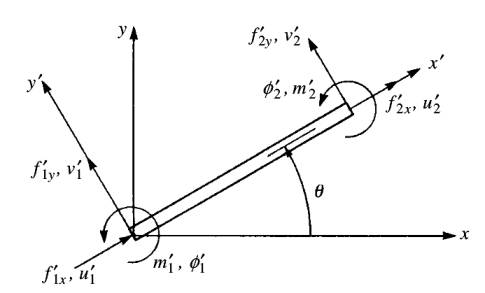
\includegraphics[width=15em]{phy_020_strs_06_02.jpg}

Önceki dersten hatırlarsak eksene dik yük alan parçaların mekaniği alttaki
formülle gösterilmişti,

$$
\left[\begin{array}{c}
f_{1y} \\ m_1 \\ f_{2y} \\ m_2
\end{array}\right] =
\frac{EI}{L^3}
\left[\begin{array}{cccc}
12 & 6L & -12 & 6L \\
6L & 4L^2 & -6L & 2L^2 \\
-12 & -6L & 12 & -6L \\
6L & 2L^2 & -6L & 4L^2
\end{array}\right]
\left[\begin{array}{ccc}
v_1 \\ \phi_1 \\ v_2 \\ \phi_2
\end{array}\right]
$$

Bu formüle (1)'deki eksenel mantığı eklersek, yerel kordinatlarda

$$
\left[\begin{array}{c}
f'_{1x} \\ f'_{1y} \\ m'_1 \\ f'_{2x} \\ f'_{2y} \\ m'_2
\end{array}\right] =
\left[\begin{array}{cccccc}
C_1 & 0 & 0 & -C_1 & 0 & 0 \\
0 & 12C_2 & 6 C_2 L & 0 & -12 C_2 & 6 C_2 L \\
0 & 6C_2 L & 4 C_2 L^2 & 0 & -6 C_2 L & 2 C_2 L^2 \\
-C_1 & 0 & 0 & C_1 & 0 & 0 \\
0 & -12C_2 & -6 C_2 L & 0 & 12 C_2 & -6 C_2 L \\
0 & 6 C_2 L & 2 C_2 L^2 & 0 & -6C_2 L & 4C_2 L^2
\end{array}\right]
\left[\begin{array}{c}
u'_1 \\ v'_1 \\ \phi'_1 \\ u'_2 \\ v'_2 \\ \phi'_2
\end{array}\right]
\mlabel{4}
$$

elde edilir, ki $C_1 = \dfrac{AE}{L}$ ve $C_2 = \dfrac{EI}{L^3}$
olmak üzere. Üstte ortada duran matris $k'$ matrisidir.

Şimdi dönüş mekaniğini ekleyelim.

$$
\left[\begin{array}{ccc}
u'_1 \\ v'_1 \\ \phi'_1 \\ u'_2 \\ v'_2 \\ \phi'_2 
\end{array}\right] =
\left[\begin{array}{cccccc}
C & S & 0 & 0 & 0 & 0 \\
-S & C & 0 & 0 & 0 & 0 \\
0 & 0 & 1 & 0 & 0 & 0 \\
0 & 0 & 0 & C & S & 0 \\
0 & 0 & 0 & -S & C & 0 \\
0 & 0 & 0 & 0 & 0 & 1
\end{array}\right]
\left[\begin{array}{ccc}
u_1 \\ v_1 \\ \phi_1 \\ u_2 \\ v_2 \\ \phi_2 
\end{array}\right]
\mlabel{5}
$$

Ortadaki matris yerel öğeler için etkili $T$ matrisi. Dikkat edersek dönüş
sağlayan 2 x 2 boyutundaki iki altmatrisler, $T$'de görülen o iki bölge, daha
büyük matriste öyle yerleştirildi ki sadece $u_1,v_1$ ve $u_2,v_2$
değişkenlerini etkiliyor, onlara tekabül eden bölgelerde duruyor.

Böylece $T$ matrisini bulmuş olduk. Şimdi $k$ matrisini hesaplamak için
$k = T^T k' T$ işlemini yapabiliriz [1, sf. 243].

\begin{minted}[fontsize=\footnotesize]{python}
from sympy import symbols, latex, simplify
from sympy.matrices import Matrix
import pickle

C,S,C1,C2,L,A,E,I = symbols("C,S,C1,C2,L,A,E,I")
kprime = Matrix([ [C1, 0, 0, -C1, 0, 0],
                  [0, 12*C2, 6*C2*L, 0, -12*C2, 6*C2*L],
                  [0, 6*C2*L, 4*C2*L**2, 0, -6*C2*L, 2*C2*L**2],
                  [-C1, 0, 0, C1, 0, 0],
                  [0, -12*C2, -6*C2*L, 0, 12*C2, -6*C2*L],
                  [0, 6*C2*L, 2*C2*L**2, 0, -6*C2*L, 4*C2*L**2]])

T = Matrix([[C,S,0,0,0,0],[-S,C,0,0,0,0],[0,0,1,0,0,0],
            [0,0,0,C,S,0],[0,0,0,-S,C,0],[0,0,0,0,0,1]])

res = T.transpose()*kprime*T
res = res.subs(C1,A*E/L) 
res = res.subs(C2,E*I/L**3)
pickle.dump(res,open("frame.pkl","wb")) # sonra lazim olacak diske kaydet
pickle.dump(kprime,open("kprime.pkl","wb"))
pickle.dump(T,open("T.pkl","wb"))
res = res / (E/L) 
print (latex(simplify(res))[:70],'...')
\end{minted}

\begin{verbatim}
\left[\begin{matrix}A C^{2} + \frac{12 I S^{2}}{L^{2}} & \frac{C S \le ...
\end{verbatim}

$$
k = 
\frac{E}{L} \times 
\left[\begin{matrix}A C^{2} + \frac{12 I S^{2}}{L^{2}} & \frac{C S \left(A L^{2} - 12 I\right)}{L^{2}} & - \frac{6 I S}{L} & - A C^{2} - \frac{12 I S^{2}}{L^{2}} & \frac{C S \left(- A L^{2} + 12 I\right)}{L^{2}} & - \frac{6 I S}{L}\\\frac{C S \left(A L^{2} - 12 I\right)}{L^{2}} & A S^{2} + \frac{12 C^{2} I}{L^{2}} & \frac{6 C I}{L} & \frac{C S \left(- A L^{2} + 12 I\right)}{L^{2}} & - A S^{2} - \frac{12 C^{2} I}{L^{2}} & \frac{6 C I}{L}\\- \frac{6 I S}{L} & \frac{6 C I}{L} & 4 I & \frac{6 I S}{L} & - \frac{6 C I}{L} & 2 I\\- A C^{2} - \frac{12 I S^{2}}{L^{2}} & \frac{C S \left(- A L^{2} + 12 I\right)}{L^{2}} & \frac{6 I S}{L} & A C^{2} + \frac{12 I S^{2}}{L^{2}} & \frac{C S \left(A L^{2} - 12 I\right)}{L^{2}} & \frac{6 I S}{L}\\\frac{C S \left(- A L^{2} + 12 I\right)}{L^{2}} & - A S^{2} - \frac{12 C^{2} I}{L^{2}} & - \frac{6 C I}{L} & \frac{C S \left(A L^{2} - 12 I\right)}{L^{2}} & A S^{2} + \frac{12 C^{2} I}{L^{2}} & - \frac{6 C I}{L}\\- \frac{6 I S}{L} & \frac{6 C I}{L} & 2 I & \frac{6 I S}{L} & - \frac{6 C I}{L} & 4 I\end{matrix}\right]
\mlabel{3}
$$

Bu sonuç [1]'deki sonuca benziyor, cebirsel olarak eşit.

$E/L$ bölümünü \verb!sympy! basitleştirmesi öncesi sistemde dışarıdan uyguladık
çünkü cebirsel düzenlemede sisteme yardım etmek istedik, bu sayede sonuç
kitaptaki çıktıya benzemiş oldu. Ayrıca cebirsel işlem sonucunu diske kaydettik
(3) çıktısı alttaki problemde lazım olacak.

Birden fazla kiriş formülü de üstdüşüm ile birleştirilerek daha büyük bir
yapının formülü haline getirilebilir, alttaki soruda bunun nasıl yapılacağını
göreceğiz. Elde edilecek sistem / matris düz katı şasi / düz oynamaz çerçeve
(rigid plane frame) formülasyonu için kullanılacak, bu sistem ``katı bir şekilde
birbirine bağlanmış bir grup kiriş parçalarının toplamı'' olarak ta tarif
edilebilir, yani kiriş parçalarının birbirine olan açıları, yük uygulandıktan
sonra bağlandıklarında ne ise o halde kalırlar, deformasyon sonrası değişime
uğramazlar. Ayrıca bu tür bir sistemde moment bir parçadan diğerine, bağlantı
noktaları üzerinden transfer olabilir, yani katı bağlantı noktaları üzerinden
bir moment sürekliliği vardır.

Soru

İlk katı düzlem çerçeve analizi olarak alttaki basit sistemi çözün.

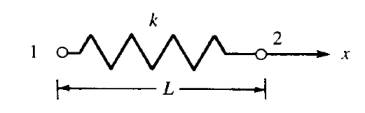
\includegraphics[width=15em]{phy_020_strs_06_03.jpg}

Cevap

Sistem düğüm 1 ve 4 üzerinden sabitlenmiş, düğüm 2 üzerinde ve yatay 40 kN
kuvvet uygulanıyor, ayrıca düğüm 3'te pozitif moment 500 N-m var. Üstteki
resimde global kordinat sisteminin yeri gösteriliyor [1, sf. 244].

Çözüm için her parçayı kiriş matematiği (3) ile formülize edeceğiz, ve bu
parçaları üstdüşüm ile biraraya koyacağız, nihai matrisi çözerek yükleri ve yer
değişimleri bulacağız.

Parça 1

Hesap yapabilmek için (3)'teki matrise ihtiyaç var, bu matrisin sembolik
halini diskten okuyalım, oraya kaydetmiştik, 

\begin{minted}[fontsize=\footnotesize]{python}
from sympy import symbols, latex, simplify
from sympy.matrices import Matrix
import pickle, pandas as pd
pd.set_option('display.max_columns', None)
pd.set_option("display.precision", 4)
C,S,L,A,E,I = symbols("C,S,L,A,E,I")
frame = pickle.load(open('frame.pkl','rb'))
\end{minted}

Birinci parçanın duruş açısı 90 derece, o zaman $C = \cos 90 = 0$, $S = \sin 90
= 1$.  Bu değerleri sembolik matrisi sayısal hale çevirmek için kullanacağız,
``yoğun (dense) matris'' elde edeceğiz, \verb!subs! çağrısı ile,

\begin{minted}[fontsize=\footnotesize]{python}
d = {L:3000.0, C:0.0, S:1.0, E:200.0*1e3, A:6500.0, I:80.0*1e6}
res = frame.subs(d) / (1e3*d[E]/d[L])
df1 = pd.DataFrame(np.array(res).astype(np.float64))
df1.columns = ['u1','v1','phi1','u2','v2','phi2']
df1 = df1.round(2)
print ('66.67*1000 * \n', df1)
\end{minted}

\begin{verbatim}
66.67*1000 * 
        u1   v1      phi1      u2   v2      phi2
0    0.11  0.0    -160.0   -0.11  0.0    -160.0
1    0.00  6.5       0.0    0.00 -6.5       0.0
2 -160.00  0.0  320000.0  160.00  0.0  160000.0
3   -0.11  0.0     160.0    0.11  0.0     160.0
4    0.00 -6.5       0.0    0.00  6.5       0.0
5 -160.00  0.0  160000.0  160.00  0.0  320000.0
\end{verbatim}

Matrisin birimi N/mm. 

Parça 2

Bu parçanın duruşu sebebiyle açı sıfır, yani $C=1,S=0$.

\begin{minted}[fontsize=\footnotesize]{python}
d = {L:3000.0, C:1.0, S:0.0, E:200.0*1e3, A:6500.0, I:40.0*1e6}
res = frame.subs(d) / (1e3*d[E]/d[L])
df2 = pd.DataFrame(np.array(res).astype(np.float64))
df2.columns = ['u2','v2','phi2','u3','v3','phi3']
print ('66.67*1000 * \n', df2)
\end{minted}

\begin{verbatim}
66.67*1000 * 
     u2       v2      phi2   u3       v3      phi3
0  6.5   0.0000       0.0 -6.5   0.0000       0.0
1  0.0   0.0533      80.0  0.0  -0.0533      80.0
2  0.0  80.0000  160000.0  0.0 -80.0000   80000.0
3 -6.5   0.0000       0.0  6.5   0.0000       0.0
4  0.0  -0.0533     -80.0  0.0   0.0533     -80.0
5  0.0  80.0000   80000.0  0.0 -80.0000  160000.0
\end{verbatim}

Parça 3

Açı 270 derece, demek ki $C=0,S=-1$.

\begin{minted}[fontsize=\footnotesize]{python}
d = {L:3000.0, C:0.0, S:-1, E:200.0*1e3, A:6500.0, I:80.0*1e6}
res = frame.subs(d) / (1e3*d[E]/d[L])
df3 = pd.DataFrame(np.array(res).astype(np.float64))
df3.columns = ['u3','v3','phi3','u4','v4','phi4']
print ('66.67*1000 * \n', df3)
\end{minted}

\begin{verbatim}
66.67*1000 * 
          u3   v3      phi3        u4   v4      phi4
0    0.1067  0.0     160.0   -0.1067  0.0     160.0
1    0.0000  6.5       0.0    0.0000 -6.5       0.0
2  160.0000  0.0  320000.0 -160.0000  0.0  160000.0
3   -0.1067  0.0    -160.0    0.1067  0.0    -160.0
4    0.0000 -6.5       0.0    0.0000  6.5       0.0
5  160.0000  0.0  160000.0 -160.0000  0.0  320000.0
\end{verbatim}

Üstteki üç matris birleştirilip, üstdüşüm üzerinden daha büyük bir matris haline
getirilecek. Üstdüşüm yapılabilmesi için her matrisin aynı boyutta, aynı
kolonlara sahip olması gerekir. Bir matrisi (ya da Dataframe) alıp yeni
değişkenlere ``büyüten'' bir kod parçası lazım.

\begin{minted}[fontsize=\footnotesize]{python}
import pandas as pd
pd.set_option('display.max_columns', None)

def expand_dataframe(df, new_cols):

    res = df.copy()
    old_cols = list(df.columns)
    addn_vars = [x for x in new_cols if x not in old_cols]
    res.index = df.columns
    for x in addn_vars:
        res[x] = np.nan
        res.loc[x] = pd.Series(res.columns)
    res = res[new_cols]
    res = res.reindex(new_cols).fillna(0)
    return res

df = pd.DataFrame([['a','c'],['b','d']],columns = ['u1','u3'])
print (df)
res = expand_dataframe(df,['u1','u2','u3','u4'])
print (res)
\end{minted}

\begin{verbatim}
  u1 u3
0  a  c
1  b  d
   u1   u2 u3   u4
u1  a  0.0  c  0.0
u2  0  0.0  0  0.0
u3  b  0.0  d  0.0
u4  0  0.0  0  0.0
\end{verbatim}

Üstteki kod parçası bunu yapabiliyor, örnek verideki ilk \verb!u1!, \verb!u3!
kolon listesini \verb!u1!, \verb!u2!, \verb!u3!, \verb!u4! listesine büyüttük,
ve kod gerekli yerlere gerekli sıfır değerlerini yazdı ve eski matrisin
değerlerini büyütülmüş yeni matriste uygun yerlere taşıdı.

Nihai matristen değişken çıkartmak ta lazım olabiliyor, sınır şartları bunu
gerektiriyor olabilir. mesela \verb!u1=0! için bu değişkene tekabül eden hem
kolon hem satır çıkartılmalı,

\begin{minted}[fontsize=\footnotesize]{python}
res2 = res.copy()
res2 = res2.drop('u1',axis=1)
res2 = res2.drop('u1',axis=0)
print (res2)
\end{minted}

\begin{verbatim}
     u2 u3   u4
u2  0.0  0  0.0
u3  0.0  d  0.0
u4  0.0  0  0.0
\end{verbatim}

Verilen bir kolon ve satırların listesini çıkartmak için de bir fonksiyon yazalım,

\begin{minted}[fontsize=\footnotesize]{python}
def drop_col_row(df, var_list):
    res = df.copy()
    for x in var_list:
        res = res.drop(x,axis=1)
        res = res.drop(x,axis=0)
    return res
\end{minted}

Son hesap aşamasına geldik. Üstdüşüm yapalım, ve $u_1 = v_1 = \phi_1 = 0$,
$u_4 = v_4 = \phi_4 = 0$ şartlarını uygulayalım,

\begin{minted}[fontsize=\footnotesize]{python}
all_vars = ['u1','v1','phi1','u2','v2','phi2','u3','v3','phi3','u4','v4','phi4']
df1f = expand_dataframe(df1,all_vars)
df2f = expand_dataframe(df2,all_vars)
df3f = expand_dataframe(df3,all_vars)
df_super = df1f + df2f + df3f

df_super = drop_col_row(df_super, ['u1','v1','phi1','u4','v4','phi4'])
print (df_super)
\end{minted}

\begin{verbatim}
          u2       v2      phi2        u3       v3      phi3
u2      6.61   0.0000     160.0   -6.5000   0.0000       0.0
v2      0.00   6.5533      80.0    0.0000  -0.0533      80.0
phi2  160.00  80.0000  480000.0    0.0000 -80.0000   80000.0
u3     -6.50   0.0000       0.0    6.6067   0.0000     160.0
v3      0.00  -0.0533     -80.0    0.0000   6.5533     -80.0
phi3    0.00  80.0000   80000.0  160.0000 -80.0000  480000.0
\end{verbatim}

Bu matrisi bir $Ax = b$ lineer sistemini çözmek için kullanacağız. Üstteki
matris $A$ olacak, $b$ ise kuvvet ve momentleri taşıyan bir vektör,
sınır şartlarının çıkarttığı değerler sonrası kalan değişkenler,

$$
\left[\begin{array}{c}
f_{2x} \\ f_{2y} \\ m_{2} \\ f_{3x} \\ f_{3y} \\ m_{3} 
\end{array}\right] =
\left[\begin{array}{c}
4 \times 10^4 \\ 0 \\ 0 \\ 0 \\ 0 \\ 5 \times 10^5
\end{array}\right]
$$

Çözeceğimiz sistem

$$
\left[\begin{array}{c}
4 \times 10^4 \\ 0 \\ 0 \\ 0 \\ 0 \\ 5 \times 10^5
\end{array}\right]
=
66.67 \times 10^3
\left[\begin{array}{cccccc}
  6.61 &  0 &     160 &   -6.5 &   0   &    0 \\
  0    & 6.5533 &  80.0 &    0 &  -0.0533 &   80.0 \\
160 &  80 &  480000 &    0 & -80 &   80000 \\
 -6.50 &   0 &       0 &    6.6067 &   0 &     160.0 \\
  0 &  -0.0533 &     -80.0 &    0 &   6.5533 &     -80.0 \\
  0 &  80 &.   80000 &  160 & -80 &  480000 
\end{array}\right]
\left[\begin{array}{c}
u_2 \\ v_2 \\ \phi_2 \\ u_3 \\ v_3 \\ \phi_3
\end{array}\right]
$$

\begin{minted}[fontsize=\footnotesize]{python}
import numpy.linalg as lin

b = np.array([4*1e4,0,0,0,0,5*1e5])

x = lin.solve(66.67*1e3*df_super, b)

pd.DataFrame(x,index=df_super.columns)
\end{minted}

\begin{verbatim}
Out[1]: 
           0
u2    4.8197
v2    0.0333
phi2 -0.0014
u3    4.7747
v3   -0.0333
phi3 -0.0014
\end{verbatim}

Birimler yer değişimleri için mm, açılar için radyan. Sonuçlara göre düğüm 2 ve
3 noktalarında şasi bir miktar sağa doğru gidiyor, ve dikey yer değişim ve dönüş
yok denecek kadar az.

Her Parçaya Etki Eden Yerel Kuvvetler

Bir kez tüm sistem bazında yer değişimlerini hesapladıktan sonra bunları
kullanarak her ögeye etki eden kuvvetleri bulabiliriz, $f' = k' T d$
gerekli. Daha önce (4)'te gösterilen $k'$ ve (5)'te gösterilen $T$ matrislerini
sembolik olarak kaydetmiştik, onları geri okuyup birinci öğe için değerleri
geçelim [1, sf. 247],

\begin{minted}[fontsize=\footnotesize]{python}
import pickle, pandas as pd
from sympy import symbols
pd.set_option("display.precision", 4)
pd.set_option('display.max_columns', None)

kprime = pickle.load(open('kprime.pkl','rb'))
T = pickle.load(open('T.pkl','rb'))
C,S,C1,C2,L,A,E,I = symbols("C,S,C1,C2,L,A,E,I")
d = {L:3000.0, C:0.0, S:1.0, E:200.0*1e3, A:6500.0, I:80.0*1e6}
kprime = kprime.subs(C1,A*E/L) 
kprime = kprime.subs(C2,E*I/L**3)
kprime = kprime.subs(d) 
kprime = pd.DataFrame(np.array(kprime),dtype=np.float64)  / (66.67*1e3)
print (kprime)

T = T.subs(C,0)
T = T.subs(S,1)
T = pd.DataFrame(np.array(T),dtype=np.float64)
print (T)
\end{minted}

\begin{verbatim}
      0      1         2     3       4         5
0  6.50   0.00      0.00 -6.50    0.00      0.00
1  0.00   0.11    159.99  0.00   -0.11    159.99
2  0.00 159.99 319984.00  0.00 -159.99 159992.00
3 -6.50   0.00      0.00  6.50    0.00      0.00
4  0.00  -0.11   -159.99  0.00    0.11   -159.99
5  0.00 159.99 159992.00  0.00 -159.99 319984.00
      0    1    2     3    4    5
0  0.00 1.00 0.00  0.00 0.00 0.00
1 -1.00 0.00 0.00  0.00 0.00 0.00
2  0.00 0.00 1.00  0.00 0.00 0.00
3  0.00 0.00 0.00  0.00 1.00 0.00
4  0.00 0.00 0.00 -1.00 0.00 0.00
5  0.00 0.00 0.00  0.00 0.00 1.00
\end{verbatim}

Birinci öğe için geçerli olan yer değişimler

$$
d = \left[\begin{array}{c}
u_1 = 0 \\ v_1 = 0 \\ \phi_1 = 0 \\ u_2 = 5.007 \\ v_2 = 0.0345 \\ \phi_2 = -0.00144
\end{array}\right]
$$

Artık $f' = k' T d$ hesaplanabilir,

\begin{minted}[fontsize=\footnotesize]{python}
d = np.array([[0,0,0,5.007,0.0345,-0.00144]]).T
fprime = 66.67*1e3 * np.dot(kprime,T).dot(d)
fprime = pd.DataFrame(fprime)
fprime.index = ['fprime1x','fprime1y','mprime1','fprime2x','fprime2y','mprime2']
print (fprime)
\end{minted}

\begin{verbatim}
                   0
fprime1x   -14950.00
fprime1y    20245.33
mprime1  38048000.00
fprime2x    14950.00
fprime2y   -20245.33
mprime2  22688000.00
\end{verbatim}

Birimler kuvvetler için Newton, momentler için Newton-mm.

Diğer ögeler için benzer hesap yapılabilir.

Seyrek Matris Kodlamasi

Bir kodlama detayından bahsedelim, gerçek dünya uygulamalarında performans için
seyrek matris teknikleri kullanmak daha iyidir, bu yazı demo amaçlı bir yöntem
seçti, fakat seyrek seçenek ile mesela matrisler sözlük ile temsil edilebilir,
olan değerlerin anahtarı vardır, diğerleri dolaylı olarak yok sayılır. Üstdüşüm
yaparken birbirine uyan anahtarların değerleri toplanır, diğerleri yine boş
kalır, bu değerler sıfırdır. $Ax=b$ çözerken her satırda mevcut anahtarların
değerleri JSON olarak ayrı sözlükler olarak alınabilir ve bu satırlar artımsal
(incremental) çözüm yapabilen bir eşlenik gradyan [2,3] koduna satır satır
geçilebilir.

Kaynaklar

[1] Logan, {\em A First Course in the Finite Element Method, 6th Ed}

[2] Bayramlı, {\em Hesapsal Bilim, Ders 2-19}

[3] Bayramlı, {\em Üstdüşümlü Matris Sistemini Çözmek}
    \url{https://burakbayramli.github.io/dersblog/sk/2024/01/beam_lattice_superposition_cg_sparse.html}

\end{document}



